\documentclass[fleqn]{article}
\usepackage[nodisplayskipstretch]{setspace}
\usepackage{amsmath, nccmath, bm}
\usepackage{amssymb}
\usepackage{enumitem}
\usepackage{graphicx}

\newcommand{\zerodisplayskip}{
	\setlength{\abovedisplayskip}{0pt}%
	\setlength{\belowdisplayskip}{0pt}%
	\setlength{\abovedisplayshortskip}{0pt}%
	\setlength{\belowdisplayshortskip}{0pt}%
	\setlength{\mathindent}{0pt}}
	
\newcommand{\norm}[1]{\left \lVert #1 \right \rVert}

\makeatletter
	\newenvironment{equationCenter}{\@fleqnfalse\begin{equation*}}{\end{equation*}}
\makeatother

\setcounter{MaxMatrixCols}{20}

\title{Homework 7}
\author{Owen Sowatzke}
\date{November 29, 2023}

\begin{document}
	\offinterlineskip
	\setlength{\lineskip}{12pt}
	\zerodisplayskip
	\maketitle
	
	\begin{enumerate}[nolistsep]
		\item On $\mathcal{P}_2(\mathbb{R})$, consider the inner product given by
		
		\begin{equation*}
			\langle p, q \rangle = \int_{0}^{1}{p(x)q(x)dx}
		\end{equation*}
		
		Apply the Gram-Schmidt Procedure to the basis $1, x, x^2$ to produce an orthonormal basis of $\mathcal{P}_2(\mathbb{R})$.
		
		Let $p_1(x) = 1$, $p_2(x) = x$, and $p_3(x) = x^2$.
		
		\begin{equation*}
			e_1(x) = \frac{p_1(x)}{\norm{p_1(x)}}
		\end{equation*}  
		
		\begin{equation*}
			\norm{p_1(x)}^2 = \langle p_1(x), p_1(x) \rangle = \int_{0}^{1}{dx} = \left.x\right\vert_{0}^{1} = 1
		\end{equation*}
		
		\begin{equation*}
			\Rightarrow \norm{p_1(x)} = 1			
		\end{equation*}
		
		\begin{equation*}
			\mathbf{\therefore e_1(x) = 1}
		\end{equation*}
		
		\begin{equation*}
			w_2(x) = p_2(x) - \langle p_2(x), e_1(x) \rangle e_1(x)
		\end{equation*}
		
		\begin{equation*}
			\langle p_2(x), e_1(x) \rangle = \int_{0}^{1}{x dx} = \left.\frac{x^2}{2}\right\vert_{0}^{1} = \frac{1}{2}
		\end{equation*}
		
		\begin{equation*}
			w_2(x) = x - \frac{1}{2}
		\end{equation*}
		
		\begin{equation*}
			\norm{w_2(x)}^2 = \langle w_2(x), w_2(x) \rangle = \int_{0}^{1}{\left(x - \frac{1}{2}\right)^{2}dx} = \int_{0}^{1}{\left(x^{2} - x + \frac{1}{4}\right)dx}
		\end{equation*}
		
		\begin{equation*}
			= \left.\left(\frac{x^3}{3} - \frac{x^2}{2} + \frac{x}{4}\right)\right\vert_{0}^{1} = \frac{1}{3} - \frac{1}{2} + \frac{1}{4} = \frac{4 - 6 + 3}{12} = \frac{1}{12}
		\end{equation*}
		
		\begin{equation*}
			\Rightarrow \norm{w_2(x)} = \frac{1}{2\sqrt{3}}
		\end{equation*}
			
		\begin{equation*}
			\therefore e_2(x) = \frac{w_2(x)}{\norm{w_2(x)}} = 2\sqrt{3}\left(x - \frac{1}{2}\right) = \mathbf{\sqrt{3}(2x - 1)}
		\end{equation*}
		
		\begin{equation*}
			w_3(x) = p_3(x) - \langle p_3(x), e_2(x) \rangle e_2(x) - \langle p_3(x), e_1(x) \rangle e_1(x)
		\end{equation*}
		
		\begin{equation*}
			\langle p_3(x), e_1(x) \rangle = \int_{0}^{1}{x^{2}dx} = \left.\frac{x^3}{3}\right\vert_{0}^{1} = \frac{1}{3}
		\end{equation*}
		
		\begin{equation*}
			\langle p_3(x), e_2(x) \rangle = \int_{0}^{1}{\sqrt{3}x^{2}(2x - 1)dx} = \sqrt{3}\int_{0}^{1}{(2x^{3} - x^2)dx}
		\end{equation*}
		
		\begin{equation*}
		 	= \sqrt{3}\left.\left(\frac{x^{4}}{2} - \frac{x^{3}}{3}\right)\right\vert_{0}^{1} = \sqrt{3}\left(\frac{1}{2} - \frac{1}{3}\right) = \sqrt{3}\left(\frac{3 - 2}{6}\right) = \frac{\sqrt{3}}{6}
		\end{equation*}
		
		\begin{equation*}
			\Rightarrow w_3(x) = x^2  - \left(\frac{\sqrt{3}}{6}\right)[\sqrt{3}(2x - 1)] - \frac{1}{3}(1)
		\end{equation*}
		
		\begin{equation*}
			 = x^2 - \frac{1}{2}(2x - 1) - \frac{1}{3} = x^2 - x + \frac{1}{6}
		\end{equation*}
		
		\begin{equation*}
			\norm{w_3(x)}^2 = \langle w_3(x), w_3(x) \rangle = \int_{0}^{1}{\left(x^2 - x + \frac{1}{6}\right)^{2}dx}
		\end{equation*}
		
		\begin{equation*}
			= \int_{0}^{1}{\left(x^4 - x^3 + \frac{x^2}{6} - x^3 + x^2 - \frac{x}{6} + \frac{x^2}{6} - \frac{x}{6} + \frac{1}{36}\right)dx}
		\end{equation*}
		
		\begin{equation*}
			= \int_{0}^{1}{\left(x^4 - 2x^3 + \frac{4x^2}{3} - \frac{x}{3} + \frac{1}{36}\right)dx}
		\end{equation*}
		
		\begin{equation*}
			= \left.\left(\frac{x^5}{5} - \frac{x^4}{2} + \frac{4x^3}{9} - \frac{x^2}{6} + \frac{x}{36}\right)\right\vert_{0}^{1}
		\end{equation*}
		
		\begin{equation*}
			= \frac{1}{5} - \frac{1}{2} + \frac{4}{9} - \frac{1}{6} + \frac{1}{36} = \frac{36 - 90 + 80 - 30 + 5}{180} = \frac{1}{180}
		\end{equation*}
		
		\begin{equation*}
			\Rightarrow \norm{w_3(x)} = \frac{1}{6\sqrt{5}}
		\end{equation*}
		
		\begin{equation*}
			\therefore e_3(x) = 6\sqrt{5}\left(x^2 - x + \frac{1}{6}\right) = \mathbf{ \sqrt{5}\left(6x^2 - 6x + 1\right)}
		\end{equation*}
		
		\pagebreak
		\item Find a polynomial $q \in \mathcal{P}_2(\mathbb{R})$ such that
		
		\begin{equation*}
			\int_{0}^{1}{p(x)(\cos{{\pi}x})dx} = \int_{0}^{1}{p(x)q(x)dx} 
		\end{equation*}
		
		for every $p \in \mathcal{P}_2(\mathbb{R})$.
		
		Define:
		
		\begin{equation*}
			\varphi(v) = \int_{0}^{1}{p(x)(\cos{{\pi}x})dx}
		\end{equation*}
		
		Using the basis vectors on $\mathcal{P}_2(\mathbb{R})$ found in problem 1, we can rewrite $\varphi(v)$ as follows:
		
		$\varphi(v) = \varphi(\langle v, e_1 \rangle e_1 + \langle v, e_2 \rangle e_2 + \langle v, e_3 \rangle e_3)$
		
		$ = \langle v, e_1 \rangle \varphi(e_1) + \langle v, e_2 \rangle \varphi(e_2) + \langle v, e_3 \rangle \varphi(e_3)$
		
		$ = \langle v, e_1(\varphi(e_1))^{*} + e_2(\varphi(e_2))^{*} + e_3(\varphi(e_3))^{*} \rangle$
		
		$\therefore$ the polynomial $q(x)$ is defined as follows:
		
		$q(x) = e_1(\varphi(e_1))^{*} + e_2(\varphi(e_2))^{*} + e_3(\varphi(e_3))^{*}$
		
		where:
		
		\begin{equation*}
			\varphi(e_1) = \int_{0}^{1}{(\cos{{\pi}x})dx} = \left.\frac{1}{\pi}sin({\pi}x)\right\vert_{0}^{1} = 0
		\end{equation*}
		
		\begin{equation*}
			\varphi(e_2) = \int_{0}^{1}{\sqrt{3}(2x - 1)(\cos{{\pi}x}dx})
		\end{equation*}
		
		\begin{equation*}
			 = 2\sqrt{3}\int_{0}^{1}{x(\cos{{\pi}x})dx} - \sqrt{3}\int_{0}^{1}{(\cos{{\pi}x})dx}
		\end{equation*}
		
		Let:
		
		\begin{equation*}
			u = x \Rightarrow du = dx
		\end{equation*}
		
		\begin{equation*}
			dv = \cos{{\pi}x} \Rightarrow v = \frac{1}{\pi}sin({\pi}x)
		\end{equation*}
		
		\begin{equation*}
			\int_{0}^{1}{x(\cos{{\pi}x})dx} = \left.\frac{x}{\pi}sin({\pi}x)\right\vert_{0}^{1} - \int_{0}^{1}{\frac{1}{\pi}sin({\pi}x)dx}
		\end{equation*}
		
		\begin{equation*}
			= \left.\left(\frac{x}{\pi}sin({\pi}x) + \frac{1}{{\pi}^2}cos({\pi}x)\right)\right\vert_{0}^{1} = -\frac{1}{{\pi}^2} - \frac{1}{{\pi}^2} = -\frac{2}{{\pi}^2}
		\end{equation*}
		
		\begin{equation*}
			\int_{0}^{1}{(\cos{{\pi}x})dx} = 0
		\end{equation*}
		
		\begin{equation*}
			\therefore \varphi(e_2) = -\frac{4\sqrt{3}}{{\pi}^2}
		\end{equation*}
		
		\begin{equation*}
			\varphi(e_3) = \int_{0}^{1}{\sqrt{5}(6x^2 - 6x + 1)(\cos{{\pi}x})dx}
		\end{equation*}
		
		\begin{equation*}
			= 6\sqrt{5}\int_{0}^{1}{x^2(\cos{{\pi}x})dx} - 6\sqrt{5}\int_{0}^{1}{x(\cos{{\pi}x})dx} + \sqrt{5}\int_{0}^{1}{(\cos{{\pi}x})dx}
		\end{equation*}
		
		Let:
		
		\begin{equation*}
			u = x^2 \Rightarrow du = 2xdx
		\end{equation*}
		
		\begin{equation*}
			dv = \cos{{\pi}x} \Rightarrow v = \frac{1}{\pi}\sin({\pi}x)
		\end{equation*}
		
		\begin{equation*}
			\int_{0}^{1}{x^2(\cos{{\pi}x})dx} = \left.\frac{x^2}{\pi}sin({\pi}x)\right\vert_{0}^{1} - \frac{2}{\pi}\int_{0}^{1}{x\sin({\pi}x)dx}
		\end{equation*}
		
		Let:
		
		\begin{equation*}
			u = x \Rightarrow du = dx
		\end{equation*}
		
		\begin{equation*}
			dv = \sin{({\pi}x)} \Rightarrow v = -\frac{1}{\pi}\cos{({\pi}x)}
		\end{equation*}
		
		\begin{equation*}
			\int_{0}^{1}{x\sin({\pi}x)dx} = -\left.\frac{x}{\pi}\cos{({\pi}x)}\right\vert_{0}^{1} + \int_{0}^{1}{\frac{1}{\pi}\cos{({\pi}x)}dx}
		\end{equation*}
		
		\begin{equation*}
			= \left.\left(-\frac{x}{\pi}\cos{({\pi}x)} + \frac{1}{{\pi}^2}{\sin{({\pi}x)}dx}\right)\right\vert_{0}^{1}
		\end{equation*}
		
		\begin{equation*}
			\Rightarrow \int_{0}^{1}{x^2(\cos{{\pi}x})dx} = \left.\left(\frac{x^2}{\pi}sin({\pi}x) + \frac{2x}{{\pi}^2}\cos{({\pi}x)} - \frac{2}{{\pi}^3}\sin{({\pi}x)}\right)\right\vert_{0}^{1} = -\frac{2}{{\pi}^2}
		\end{equation*}
		
		\begin{equation*}
			\int_{0}^{1}{x(\cos{{\pi}x})dx} = -\frac{2}{{\pi}^2}
		\end{equation*}
		
		\begin{equation*}
			\int_{0}^{1}{(\cos{{\pi}x})dx} = 0
		\end{equation*}
		
		\begin{equation*}
			\therefore \varphi(e_3) = 6\sqrt{5}\left(-\frac{2}{{\pi}^2}\right) - 6\sqrt{5}\left(-\frac{2}{{\pi}^2}\right) = 0
		\end{equation*}
		
		\begin{equation*}
			\mathbf{\therefore q(x) = -\frac{12}{{\pi}^2}(2x - 1)}
		\end{equation*}
		
		\item In $\mathbb{R}^4$, let
		
		$U = \text{span}((1,1,0,0),(1,1,1,2))$
		
		Find $u \in U$ such that $\norm{u - (1,2,3,4)}$ is a small as possible.
		
		Find the orthonormal basis vectors of $U$.
		
		\begin{equation*}
			e_1 = \frac{u_1}{\norm{u_1}}
		\end{equation*}
		
		\begin{equation*}
			\norm{u_1}^2 = \langle u_1, u_1 \rangle = 1 + 1 + 0 + 0 = 2
		\end{equation*}
		
		\begin{equation*}
			\Rightarrow \norm{u_1} = \sqrt{2} 
		\end{equation*}
		
		\begin{equation*}
			\therefore e_1 = \frac{1}{\sqrt{2}}\begin{bmatrix}1\\1\\0\\0\end{bmatrix}
		\end{equation*}
		
		\begin{equation*}
			w_2 = u_2 - \langle u_2, e_1 \rangle e_1
		\end{equation*}
		
		\begin{equation*}
			\langle u_2, e_1 \rangle = \frac{1}{\sqrt{2}} + \frac{1}{\sqrt{2}} = \frac{2}{\sqrt{2}}
		\end{equation*}
		
		\begin{equation*}
			w_2 = \begin{bmatrix}1\\1\\1\\2\end{bmatrix} - \begin{bmatrix}1\\1\\0\\0\end{bmatrix} = \begin{bmatrix}0\\0\\1\\2\end{bmatrix}
		\end{equation*}
		
		\begin{equation*}
			\norm{w_2}^2 = \langle w_2, w_2 \rangle = 0 + 0 + 1 + 4 = 5
		\end{equation*}
		
		\begin{equation*}
			\Rightarrow \norm{w_2} = \sqrt{5} 
		\end{equation*}
		
		\begin{equation*}
			\therefore e_2 = \frac{w_2}{\norm{w_2}} = \frac{1}{\sqrt{5}}\begin{bmatrix}0\\0\\1\\2\end{bmatrix}
		\end{equation*}
		
		Let $v = (1,2,3,4)$.
		
		To minimize the distance between $u$ and $v$, let $u = P_{U}v$.
		
		$u = P_{U}v = \langle v, e_1 \rangle e_1 + \langle v, e_2 \rangle e_2$
		
		\begin{equation*}
			\langle v, e_1 \rangle = \frac{1}{\sqrt{2}} + \frac{2}{\sqrt{2}} = \frac{3}{\sqrt{2}}
		\end{equation*}
		
		\begin{equation*}
			\langle v, e_2 \rangle = \frac{3}{\sqrt{5}} + \frac{8}{\sqrt{5}} = \frac{11}{\sqrt{5}}
		\end{equation*}
		
		\begin{equation*}
			\therefore u = \frac{3}{2}\begin{bmatrix}1\\1\\0\\0\end{bmatrix} + \frac{11}{5}\begin{bmatrix}0\\0\\1\\2\end{bmatrix} = \mathbf{\frac{1}{10}\pmb{\begin{bmatrix}15\\15\\22\\44\end{bmatrix}}}
		\end{equation*}
		
		\item Suppose $T \in \mathcal{L}(V,W)$. Prove that
		
		\begin{enumerate}[nolistsep]
			\item $T$ is injective if and only if $T^\dag$ is surjective;
			\item $T$ is surjective if and only if $T^\dag$ is injective. 
		\end{enumerate}
		
		$T$ is injective $\Leftrightarrow \text{null}\ T = \{0\}$
		
		$\Leftrightarrow (\text{range}\ T^{\dag})^{\perp} = \{0\}$
		
		$\Leftrightarrow \text{range}\ T^{\dag} = W$
		
		$\Leftrightarrow T^{\dag}$ is surjective
		
		$T$ is surjective $\Leftrightarrow \text{range}\ T = W$
		
		$\Leftrightarrow (\text{null}\ T^{\dag})^{\perp} = W$
		
		$\Leftrightarrow \text{null}\ T^{\dag} = \{0\}$
		
		$\Leftrightarrow T^{\dag}$ is injective
		
		\item \textbf{Markov Chain:} Consider a system with $N$ possible states that evolves in discrete time steps. If the transition from one state, $a$, to another state, $b$, is a purely random event that occurs with probability $P_{ab}$, then the system is known as a \textit{Markov Chain}, or \textit{Finite State Machine}. Note that the probabilistic definition means that the evolution of the system is independent of the prior states of the system (not counting the current state). For this reason, Markov Chains are said to be \textit{memoryless}.
		
		Consider the case with $N=3$. The transition probabilities can be collected in matrix form as:
		
		\begin{equationCenter}
			T = \begin{bmatrix}
				P_{11} & P_{21} & P_{31} \\
				P_{12} & P_{22} & P_{32} \\
				P_{13} & P_{23} & P_{33}
			\end{bmatrix}
		\end{equationCenter}
		
		Here, the notation $P_{12}$ means "the probability that a system in state one transitions to state
two." Note that the numbers in any column of the matrix must sum to 1, since these numbers correspond to the sum of all possible transition probabilities from a given state.

		Now imagine that we don't have exact knowledge of the starting state of the system, but only know the relative probabilities of the different states. These probabilities can be collected in a vector
		
		\begin{equationCenter}
			v_0 = \begin{bmatrix}
				P_1 \\ P_2 \\ P_3
			\end{bmatrix}
		\end{equationCenter}
		
		Note that the elements in $v_0$ must also sum to 1.
		
		\begin{enumerate}
			\item Show that the update procedure for the probabilistic state description can be written as:
			
			\begin{equationCenter}
				v_n = Tv_{n-1}
			\end{equationCenter}
			
			Note that, given our definitions of matrix multiplication, this means that time evolution by one time step is a linear operator, which has the matrix representation $T$ in the standard basis.
			
			The update procedure can be expanded as follows:
			
			\begin{equation*}
				\begin{bmatrix}
					P_{1}^{n} \\
					P_{2}^{n} \\
					P_{3}^{n}
				\end{bmatrix} = \begin{bmatrix}
					P_{11} & P_{21} & P_{31} \\
					P_{12} & P_{22} & P_{32} \\
					P_{13} & P_{23} & P_{33}
				\end{bmatrix}\begin{bmatrix}
					P_{1}^{n-1} \\
					P_{2}^{n-1} \\
					P_{3}^{n-1}
				\end{bmatrix}
			\end{equation*}
			
			Each of the state probabilities can be expressed as follows:
			
			\begin{equation*}
				\begin{cases}
					P_{1}^{n} = P_{11}P_{1}^{n-1} + P_{21}P_{2}^{n-1} + P_{31}P_{3}^{n-1} \\
					P_{2}^{n} = P_{12}P_{1}^{n-1} + P_{22}P_{2}^{n-1} + P_{32}P_{3}^{n-1} \\
					P_{3}^{n} = P_{13}P_{1}^{n-1} + P_{23}P_{2}^{n-1} + P_{33}P_{3}^{n-1}
				\end{cases}
			\end{equation*}
			
			Note each of the above equations is simply a restatement of the theorem of total probability.
			
			\begin{equation*}
				P(A) = \sum_{n}{P(A|B_n)P(B_n)}
			\end{equation*}
			
			This is the expected result. Therefore, the update procedure can be written as $v_n = Tv_{n-1}$.
			
			\item Show that if $T$ and $v_0$ start properly normalized, that the state vector at any time step is also properly normalized.
			
			For the state vector to be properly normalized, the sum of each of its elements must equal 1.
			
			\begin{equation*}
				Tv_0 = \begin{bmatrix}
					P_{11} & P_{21} & P_{31} \\
					P_{12} & P_{22} & P_{32} \\
					P_{13} & P_{23} & P_{33}
				\end{bmatrix}\begin{bmatrix}
					P_1 \\
					P_2 \\
					P_3
				\end{bmatrix}
			\end{equation*}
			
			Consider the sum of the elements in $Tv_0$:
			
			$(P_{11}P_{1} + P_{21}P_{2} + P_{31}P_{3}) + (P_{12}P_{1} + P_{22}P_{2} + P_{32}P_{3})$
			
			$ + (P_{13}P_{1} + P_{23}P_{2} + P_{33}P_{3})$
			
			$ = P_{1}(P_{11} + P_{12} + P_{13}) + P_{2}(P_{21} + P_{22} + P_{23}) + P_{3}(P_{31} + P_{32} + P_{33})$
			
			$ = P_{1} + P_{2} + P_{3} = 1$
			
			$\therefore$, the state vector at the next time step is properly normalized. Note, by the same proof, the state vector at the next time step will also be properly normalized. By induction, we can conclude that the state vector at any time step will be properly normalized.
			 
			\item Consider the specific case where
			
			\begin{equationCenter}
				T = \begin{bmatrix}
					0.6 & 0.3 & 0.1\\
					0.2 & 0.2 & 0.5\\
					0.2 & 0.5 & 0.4
				\end{bmatrix}
			\end{equationCenter}
			
			Compute the operator for time evolution by \textit{three} timesteps.
			
			\begin{equation*}
				T^3 = \begin{bmatrix}
					0.6 & 0.3 & 0.1\\
					0.2 & 0.2 & 0.5\\
					0.2 & 0.5 & 0.4
				\end{bmatrix}\begin{bmatrix}
					0.6 & 0.3 & 0.1\\
					0.2 & 0.2 & 0.5\\
					0.2 & 0.5 & 0.4
				\end{bmatrix}\begin{bmatrix}
					0.6 & 0.3 & 0.1\\
					0.2 & 0.2 & 0.5\\
					0.2 & 0.5 & 0.4
				\end{bmatrix}
			\end{equation*}
			
			\begin{equation*}
				= \begin{bmatrix}
					0.44 & 0.29 & 0.25\\
					0.26 & 0.35 & 0.32\\
					0.3  & 0.36 & 0.43
				\end{bmatrix}\begin{bmatrix}
					0.6 & 0.3 & 0.1\\
					0.2 & 0.2 & 0.5\\
					0.2 & 0.5 & 0.4
				\end{bmatrix} = \pmb{\begin{bmatrix}
					0.372 & 0.315 & 0.289\\
					0.29  & 0.308 & 0.329\\
					0.338 & 0.377 & 0.382
				\end{bmatrix}}
			\end{equation*}
			
			\item Using the same specific $T$, compute $v_{\infty}$. Be clever and use MATLAB to apply what you learned in a previous homework assignment.
			
			As the number of applications of $T$ approaches $\infty$, the state vector will converge to the eigenvector corresponding to the largest eigenvalue (This is true for any initial state vector).
			
			Find the eigenvalues and eigenvectors of $T$ using MATLAB:
			
			The eigenvalues of $T$ are $\lambda_1 = 1$, $\lambda_2 = 0.4162$, and $\lambda_3 = -0.2162$. The corresponding eigenvectors are
			
			\begin{equation*}
				v_1 = \begin{bmatrix}
					0.5596 \\
					0.5353 \\
					0.6326 \\
				\end{bmatrix}, 
				v_2 = \begin{bmatrix}
					0.8129 \\
					-0.3405 \\
					-0.4724 \\
				\end{bmatrix},
				v_3 = \begin{bmatrix}
					0.2209 \\
					-0.7912 \\
					0.5703
				\end{bmatrix}
			\end{equation*}
				
			$\therefore v_1$ will correspond to the final state vector. Note that we must normalizes $v_1$ for it to be a valid state vector.
			
			$0.5596 + 0.5353 + 0.6326 = 1.7275$
			
			\begin{equation*}
				v_{\infty} = \frac{1}{1.7275}\begin{bmatrix}
					0.5596 \\
					0.5353 \\
					0.6326
				\end{bmatrix} = \pmb{\begin{bmatrix}
					0.3239 \\
					0.3099 \\
					0.3662
				\end{bmatrix}}
			\end{equation*}
			
			\item Explain, in terms of how application of $T$ modifies state probabilities, why this is a such a special set of probabilities. Make sure you discuss the connection to an invariant subspace.
			
			The solution of the previous section was an eigenvector, which does not change direction upon application of $T$. In other words, the solution is an element of an invariant subspace. Because the result will always be normalized, the solution also remains at a fixed value.
		\end{enumerate}
		
		\item \textbf{Game Strategy:} Consider a multiplayer board game that takes place on the following board and with the following rules:
		
		\begin{minipage}{\linewidth}
    			\centerline{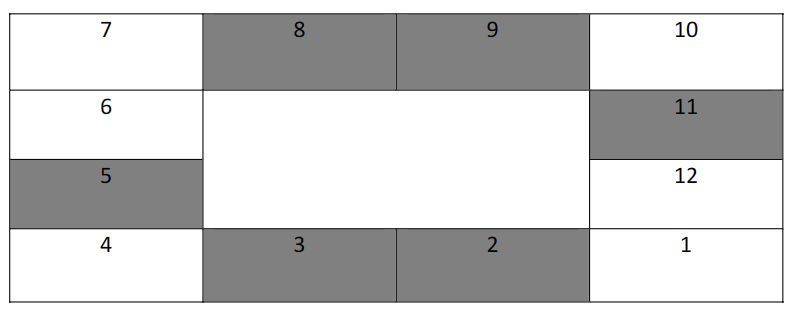
\includegraphics[scale=0.8]{monopoly_board.png}}
  		\end{minipage}	
		
		The board contains six squares that are “property” (the shaded squares) and six squares that are “not property” (the un-shaded squares).
		
		\begin{enumerate}
			\item The game starts with the players on square 1. Each player starts with a fixed number of points (money). The specific number of points (money) does not matter.
			
			\item When it is a player’s turn, they roll a single, six-sided die and move forward that many squares from their current position.

			\item If a player ends their turn on an unowned property square, they may choose to purchase that property, provided they have enough points (money) to do so. All property squares have the same cost (the specific cost does not matter).

			\item If a player ends their turn on a property square that is already owned, that player must pay a penalty to the owner of the property (the specific value of the penalty does not matter). If a player does not have enough points (money) to pay the penalty, they are out of the game.
			
			\item When a player reaches (or passes) square one, they receive bonus points (the specific value of the bonus does not matter).

			\item Play continues until all the players except one have been eliminated. The remaining player is the winner of the game.

			\item No turn can end on square 10. If a player’s roll would have them finish their turn on square 10, then they move to square 4 and end their turn at square 4.

			\item If a player’s roll would have them finish their turn on squares 6 or 12, then they draw a card from a small deck of cards. The card indicates a “special” event that happens to that player. The majority of the cards only affect the player’s point (money) total and the player ends their turn on that square. However, there is a 5\% chance of drawing a card that indicates that the player should move to square 1. In this case, the player moves to square 1, collects the relevant bonus, and ends their turn at square 1.

			(Some of you may recognize the above game as a very simplified version of the game \textit{Monopoly.})

			Obviously, you must own properties to win the game. But which properties should one own? The different properties will have different impacts on the probability of your eventual victory. Use the tools you have learned in this course to develop a simple strategy for this game. Specifically, rank the properties in the order of how beneficial they would be for you to own in your quest to win the game. (Rank the properties from the most beneficial property to the least beneficial.) Be sure to explain the methodology by which you arrived at your strategy.
			
			\textbf{HINT:} Assume the various costs/penalties/etc. are such that the players will circle the board many times before being eliminated from the game.
			
			\textbf{HINT 2:} Think of a player’s location as their “state.” How are different states connected? Think back to earlier homework problems for inspiration.
			
			We can view each player's position as a Markov chain, where the state vector determines the probability of a player being on a given tile during their turn. The best properties to own are the properties that players are most likely to land on. Because the players will circle the board many times, we are interested in the state vector, $v_{\infty}$. We can solve for the probabilities in this state vector by doing an eigenvalue decomposition of the transition matrix. The eigenvector corresponding to the largest eigenvalue should give us, $v_\infty$. To determine the best properties to buy, we simply need to sort the elements of this state vector from largest to smallest (ignoring non-property tiles).
			
			Considering the effects from part (b) alone, the transition matrix $T$ will be given by:
			
			\begin{equation*}
				T = \begin{bmatrix}
					0 & 0 & 0 & 0 & 0 & 0 & \frac{1}{6} & \frac{1}{6} & \frac{1}{6} & \frac{1}{6} & \frac{1}{6} & \frac{1}{6}\\[3pt]
					\frac{1}{6} & 0 & 0 & 0 & 0 & 0 & 0 & \frac{1}{6} & \frac{1}{6} & \frac{1}{6} & \frac{1}{6} & \frac{1}{6}\\[3pt]
					\frac{1}{6} & \frac{1}{6} & 0 & 0 & 0 & 0 & 0 & 0 & \frac{1}{6} & \frac{1}{6} & \frac{1}{6} & \frac{1}{6}\\[3pt]
					\frac{1}{6} & \frac{1}{6} & \frac{1}{6} & 0 & 0 & 0 & 0 & 0 & 0 & \frac{1}{6} & \frac{1}{6} & \frac{1}{6}\\[3pt]
					\frac{1}{6} & \frac{1}{6} & \frac{1}{6} & \frac{1}{6} & 0 & 0 & 0 & 0 & 0 & 0 & \frac{1}{6} & \frac{1}{6}\\[3pt]
					\frac{1}{6} & \frac{1}{6} & \frac{1}{6} & \frac{1}{6} & \frac{1}{6} & 0 & 0 & 0 & 0 & 0 & 0 & \frac{1}{6}\\[3pt]
					\frac{1}{6} & \frac{1}{6} & \frac{1}{6} & \frac{1}{6} & \frac{1}{6} & \frac{1}{6} & 0 & 0 & 0 & 0 & 0 & 0\\[3pt]
					0 & \frac{1}{6} & \frac{1}{6} & \frac{1}{6} & \frac{1}{6} & \frac{1}{6} & \frac{1}{6} & 0 & 0 & 0 & 0 & 0\\[3pt]
					0 & 0 & \frac{1}{6} & \frac{1}{6} & \frac{1}{6} & \frac{1}{6} & \frac{1}{6} & \frac{1}{6} & 0 & 0 & 0 & 0\\[3pt]
					0 & 0 & 0 & \frac{1}{6} & \frac{1}{6} & \frac{1}{6} & \frac{1}{6} & \frac{1}{6} & \frac{1}{6} & 0 & 0 & 0\\[3pt]
					0 & 0 & 0 & 0 & \frac{1}{6} & \frac{1}{6} & \frac{1}{6} & \frac{1}{6} & \frac{1}{6} & \frac{1}{6} & 0 & 0\\[3pt]
					0 & 0 & 0 & 0 & 0 & \frac{1}{6} & \frac{1}{6} & \frac{1}{6} & \frac{1}{6} & \frac{1}{6} & \frac{1}{6} & 0
				\end{bmatrix}
			\end{equation*}
			
			Now modify the transition matrix to account for part (g).
			
			\begin{equation*}
				T = \begin{bmatrix}
					0 & 0 & 0 & 0 & 0 & 0 & \frac{1}{6} & \frac{1}{6} & \frac{1}{6} & \frac{1}{6} & \frac{1}{6} & \frac{1}{6}\\[3pt]
					\frac{1}{6} & 0 & 0 & 0 & 0 & 0 & 0 & \frac{1}{6} & \frac{1}{6} & \frac{1}{6} & \frac{1}{6} & \frac{1}{6}\\[3pt]
					\frac{1}{6} & \frac{1}{6} & 0 & 0 & 0 & 0 & 0 & 0 & \frac{1}{6} & \frac{1}{6} & \frac{1}{6} & \frac{1}{6}\\[3pt]
					\frac{1}{6} & \frac{1}{6} & \frac{1}{6} & \frac{1}{6} & \frac{1}{6} & \frac{1}{6} & \frac{1}{6} & \frac{1}{6} & \frac{1}{6} & \frac{1}{6} & \frac{1}{6} & \frac{1}{6}\\[3pt]
					\frac{1}{6} & \frac{1}{6} & \frac{1}{6} & \frac{1}{6} & 0 & 0 & 0 & 0 & 0 & 0 & \frac{1}{6} & \frac{1}{6}\\[3pt]
					\frac{1}{6} & \frac{1}{6} & \frac{1}{6} & \frac{1}{6} & \frac{1}{6} & 0 & 0 & 0 & 0 & 0 & 0 & \frac{1}{6}\\[3pt]
					\frac{1}{6} & \frac{1}{6} & \frac{1}{6} & \frac{1}{6} & \frac{1}{6} & \frac{1}{6} & 0 & 0 & 0 & 0 & 0 & 0\\[3pt]
					0 & \frac{1}{6} & \frac{1}{6} & \frac{1}{6} & \frac{1}{6} & \frac{1}{6} & \frac{1}{6} & 0 & 0 & 0 & 0 & 0\\[3pt]
					0 & 0 & \frac{1}{6} & \frac{1}{6} & \frac{1}{6} & \frac{1}{6} & \frac{1}{6} & \frac{1}{6} & 0 & 0 & 0 & 0\\[3pt]
					0 & 0 & 0 & 0 & 0 & 0 & 0 & 0 & 0 & 0 & 0 & 0\\[3pt]
					0 & 0 & 0 & 0 & \frac{1}{6} & \frac{1}{6} & \frac{1}{6} & \frac{1}{6} & \frac{1}{6} & \frac{1}{6} & 0 & 0\\[3pt]
					0 & 0 & 0 & 0 & 0 & \frac{1}{6} & \frac{1}{6} & \frac{1}{6} & \frac{1}{6} & \frac{1}{6} & \frac{1}{6} & 0
				\end{bmatrix}
			\end{equation*}
			
			Now consider the effects of part (h). 5\% of turns that would end on square 6 or square 12, end up on square 1 instead. Therefore, row 1 of the transition matrix needs to be incremented by row 6 scaled by $\frac{1}{20}$ and row 12 scaled by $\frac{1}{20}$. Then, each entry in row 6 and row 12 needs to be scaled by $\frac{19}{20}$. The resulting transition matrix $T$ is shown below:
			
			\begin{equation*}
				T = \begin{bmatrix}
					\frac{1}{120} & \frac{1}{120} & \frac{1}{120} & \frac{1}{120} & \frac{1}{120} & \frac{1}{120} & \frac{21}{120} & \frac{21}{120} & \frac{21}{120} & \frac{21}{120} & \frac{21}{120} & \frac{21}{120}\\[3pt]
					\frac{1}{6} & 0 & 0 & 0 & 0 & 0 & 0 & \frac{1}{6} & \frac{1}{6} & \frac{1}{6} & \frac{1}{6} & \frac{1}{6}\\[3pt]
					\frac{1}{6} & \frac{1}{6} & 0 & 0 & 0 & 0 & 0 & 0 & \frac{1}{6} & \frac{1}{6} & \frac{1}{6} & \frac{1}{6}\\[3pt]
					\frac{1}{6} & \frac{1}{6} & \frac{1}{6} & \frac{1}{6} & \frac{1}{6} & \frac{1}{6} & \frac{1}{6} & \frac{1}{6} & \frac{1}{6} & \frac{1}{6} & \frac{1}{6} & \frac{1}{6}\\[3pt]
					\frac{1}{6} & \frac{1}{6} & \frac{1}{6} & \frac{1}{6} & 0 & 0 & 0 & 0 & 0 & 0 & \frac{1}{6} & \frac{1}{6}\\[3pt]
					\frac{19}{120} & \frac{19}{120} & \frac{19}{120} & \frac{19}{120} & \frac{19}{120} & 0 & 0 & 0 & 0 & 0 & 0 & \frac{19}{120}\\[3pt]
					\frac{1}{6} & \frac{1}{6} & \frac{1}{6} & \frac{1}{6} & \frac{1}{6} & \frac{1}{6} & 0 & 0 & 0 & 0 & 0 & 0\\[3pt]
					0 & \frac{1}{6} & \frac{1}{6} & \frac{1}{6} & \frac{1}{6} & \frac{1}{6} & \frac{1}{6} & 0 & 0 & 0 & 0 & 0\\[3pt]
					0 & 0 & \frac{1}{6} & \frac{1}{6} & \frac{1}{6} & \frac{1}{6} & \frac{1}{6} & \frac{1}{6} & 0 & 0 & 0 & 0\\[3pt]
					0 & 0 & 0 & 0 & 0 & 0 & 0 & 0 & 0 & 0 & 0 & 0\\[3pt]
					0 & 0 & 0 & 0 & \frac{1}{6} & \frac{1}{6} & \frac{1}{6} & \frac{1}{6} & \frac{1}{6} & \frac{1}{6} & 0 & 0\\[3pt]
					0 & 0 & 0 & 0 & 0 & \frac{19}{120} & \frac{19}{120} & \frac{19}{120} & \frac{19}{120} & \frac{19}{120} & \frac{19}{120} & 0
				\end{bmatrix}
			\end{equation*}
			
			If we perform an eigenvalue decomposition of $T$, the eigenvector corresponding to the largest eigenvalue is given by:
			
			\begin{equation*}
				v = \begin{bmatrix}
					0.2594 \\ 
					0.2264 \\
					0.2133 \\
					0.5313 \\
					0.2844 \\
					0.2761 \\
					0.2985 \\
					0.3050 \\
					0.3181 \\
					0 \\
					0.2470\\
					0.2287
				\end{bmatrix}
			\end{equation*}
			
			Because the state vector represents the probability of being on a given tile at an instant in time. We must normalize the eigenvector so that the sum of its entries is 1. After normalization, the resulting eigenvector is the equivalent to $v_{\infty}$.
			
			 \begin{equation*}
			 	v_{\infty} = \begin{bmatrix}
			 		0.0814 \\
			 		0.0710 \\
			 		0.0669 \\
			 		0.1667 \\
			 		0.0892 \\
			 		0.0866 \\
			 		0.0936 \\
			 		0.0957 \\
			 		0.0998 \\
			 		0 \\
			 		0.0775 \\
			 		0.0717
			 	\end{bmatrix}
			 \end{equation*}			
			 If we sort the entries in the final state vector, we should be able to rank the properties in order of how beneficial they are to own. Looking at $v_{\infty}$, we determine the following ordering: $\mathbf{\{9, 8, 5, 11, 2, 3\}}.$
		\end{enumerate}
	\end{enumerate}
\end{document}